\chapter{Intelligence Artificielle}

\section{Stratégies}

\subsection{Intelligence Aléatoire}

L’ IA contrôle une liste de personnages appartenant au joueur actuel,
elle va les sélectionner les uns après les autres lors de son tour 
de jeu.
Une fois un personnage sélectionné, un entier correspondant à une 
action précise est choisi au hasard parmi 6 : 1 (attaquer), 2 (se 
déplacer), 3 (utiliser un objet), 4 (défendre), 5 (utiliser une 
compétence) et 6 (passer son tour).
\\\\
Lorsqu'une action est séléctionnée on teste sa faisabilité, sinon un 
nouveau nombre est séléctionné jusqu'à ce que l'action soit valide. 
\\\\
Si l'action est possible alors elle est ajoutée à la liste des 
commandes et l'IA passe au personnage suivant.
\\\\
Si "attaquer" est choisie, une cible va être déterminée aléatoirement
parmi tout les autres personnages, y compris ceux de son équipe. Si 
la cible de l'attaque est trop éloignée alors l’attaque n’aura pas 
lieu, si la distance entre les deux personnages est suffisante alors 
l'attaque est ajoutée à la liste des commandes.
\\\\
Si "se déplacer" est choisie, le personnage sélectionné tente de se 
mouvoir sur une case aléatoire, si cela est réalisable alors le 
déplacement est ajouté à la liste des commandes.
\\\\
Si "utiliser un objet" est choisie, alors le personnage va utiliser 
un objet aléatoire de la liste des objets appartenant à son équipe, 
puis il applique l'effet sur une cible aléatoire, si l'objet est en 
quantité suffisante alors l'action est ajoutée à la liste des 
commandes.
\\\\
Si "défendre" est choisie, le personnage sélectionné se met en 
position défensive, dans le cas présent puisque l'on cherche les 
actions des personnages dans l'ordre, cette action ne peut échouer 
puisque le personnage n'a pas d'autres actions dans la liste, 
l'action "défendre" est donc ajoutée à la liste.
\\\\
Si "utiliser une compétence" est choisie, alors le personnage va 
utiliser une compétence aléatoire de la liste des compétance qu'il 
peut utiliser, puis il applique l'effet sur une cible aléatoire, si 
la distance entre lui et sa cible est inférieure à la distance 
maximum de la compétence alors la compétence est ajoutée à la liste 
des commandes.
\\\\
Si "passer son tour" est choisie, l'IA termine son tour d’action.
Lorsque passer son tour ou lorsque tout les personnages de l'équipe 
du joueur actuel ont une action, alors cela fini ainsi la liste des 
commandes, les commandes sont exécutées dans l'ordre de la liste. 
Puis c'est au tour de l'adversaire.
\\

\subsection{Intelligence Heuristique}

L'IA heuristique va lister les actions possibles par personnages 
de son équipe et calculer un score pour chacune de ces actions.
Le score est calculé en fonction de la pertinence des actions.
\\\\
Concrètement, un personnage peut se déplacer puis effectuer une action 
ou seulement effectuer une action.
Il privilégiera des déplacements où les personnages adverses ne peuvent
pas l'atteindre après déplacement ou bien s'il peut attaquer un ennemi
avec un minimum d'attaque subit le tour suivant.
\\\\
Une attaque est privilégiée si l'ennemi est tué en conséquence de
l'action. Elle est priviligié si le personnage ne peut subir que peu 
d'attaques au prochain tour, sinon l'IA privilégie la défense qui réduit
grandement les dégats subits au prochain tour adverse.
\\\\
Un objet de soin n'est utilisé que lorsque celui-ci est nécessaire 
(vie<20\% ou mana<20\%) afin qu'il ne soit pas utilisé sur des cibles 
qui n'ont pas perdu des points de vie ou des points de mana comme 
pourrait le faire l'IA aléatoire.
\\
\subsection{Intelligence Profonde}

L'IA profonde va lister les actions possibles par personnages 
de son équipe et calculer un score pour chacune de ces actions, comme le
fait l'IA heuristique. 
\\\\
On finit dans un premier temps le tour en cours en complétant la séquence
actuellement obtenue de l'IA profonde, par celle que l'on obtiendrait de
l'IA Heuristique.
\\\\
Le score est calculé après 2 tours de chaque équipe en considérant que
ces tours sont exécutés par l'intelligence heuristique, c'est-à-dire que
les tours sont réalisés dans l'optique d'obtenir les meilleures actions
possibles pour le tour.
\\\\
On calcule le score en fonction des dégâts subis par l'équipe du joueur
et ceux subis par l'adversaire.
\\\\
Après le calcul du score on exécute les tours ainsi effectués dans le
sens inverse pour revenir au tour initial.
\\\\
Cette boucle est ainsi exécutée jusqu'à ce que plus aucun personnage ne 
puisse effectué d'actions. On exécute alors la liste des commandes
obtenues avec les meilleurs scores.

\section{Conception Logiciel}
Le diagramme des classes UML C++ pour l'intelligence artificielle est
visible en Figure 5.1.
On divise l'intelligence artificielle en 4 classes.
\\
\begin{itemize}

\item \textbf{AI :} C'est la classe principale, elle définie les 
méthodes qui serviront lors du polymorphisme lorsque les 
différentes IA seront appelées.
\\
\item \textbf{RandomAI :} C'est la classe représentant l'IA 
aléatoire, elle a une fonction pour determiner la liste des actions \\
des personnages controllé par l'IA (randomCommandList) et une 
fonction pour executer lancer l'IA (runAI).
\\
\item \textbf{HeuristicAI :} C'est la classe dédiée à l'IA heurisitique.
Elle comporte une fonction computeScore qui renvoie le score calculé
pour l'action donnée en entrée, une fonction heuristicCommandList pour
déterminer la liste des actions à partir des scores et une fonction
runAI pour lancer l'IA.
\\
\item \textbf{DeepAI :} C'est la classe de l'IA profonde. Elle comporte 
une fonction minMax qui renvoie le score en considérant le meilleur tour
de l'adversaire puis le meilleur tour du joueur (2 fois). Elle comporte 
aussi une fonction deepCommandList pour déterminer la liste des actions 
à partir des scores et une fonction runAI pour lancer l'IA. 

\end{itemize}


\begin{figure}[H]
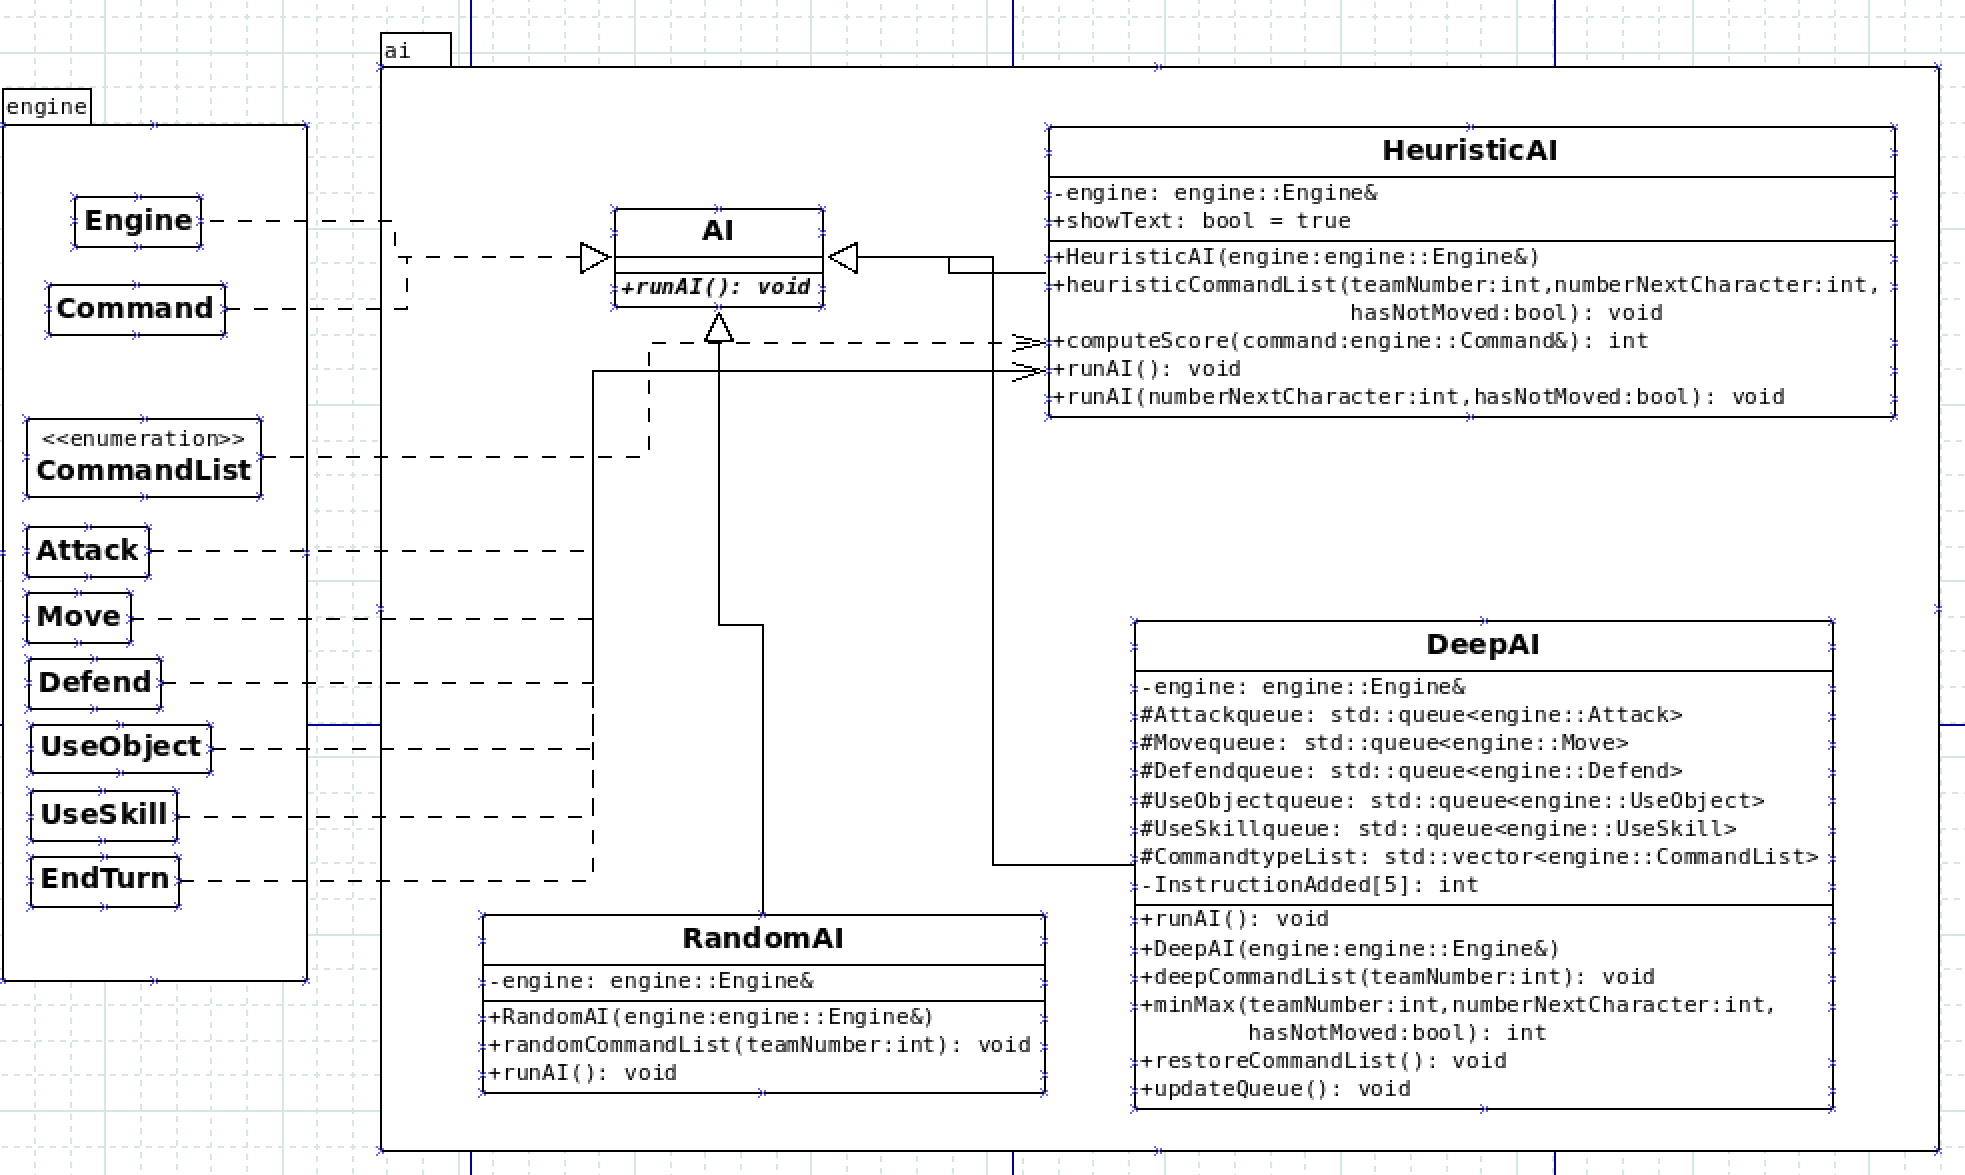
\includegraphics[width=\linewidth]{images/deep_ai_dia.png}
\centering
\caption{Aperçu de ai.dia avec HeuristicAI et DeepAI}
\label{fig:img3}
\end{figure}
\newpage
